\chapter{مقدمه ای بر الگوریتم \lr{A*}}

\section{اهمیت مسیریابی بهینه در سیستم های حمل و نقل خودران}
توسعه سیستم‌های اتومات مانند هواپیماهای بدون سرنشین، وسایل نقلیه هدایت‌شونده خودکار و ربات‌های خودکار مزایای بسیاری را برای انسان داشته اند . توسعه وسایل نقلیه خودران منجر به افزایش ایمنی جاده ها و بهبود مصرف انرژی شده است. برای خودران سازی وسایل نقلیه باید نوعی سیستم داشت تا مسیرهای خود را مطابق با محیطی که قرار است در آن حرکت کنند برنامه ریزی کند. خواسته ی ما در این گونه مسائل این است که  این مسیرها تا حد امکان کوتاه باشند و وسیله نقلیه به راحتی حرکت کند و از همه مهمتر اینکه بدون مانع باشند .
با این حال، تحقیق در مورد برنامه ریزی حرکتی سیستم های خودران جدید نیست و به دهه 1950 برمی گردد، با الگوریتم هایی مانند جستجوی عرضی و جستجوی عمقی در مرحله اولیه تحقیقات برنامه ریزی حرکتی فرموله شده است. از آن زمان تاکنون چندین پیشرفت بزرگ در توسعه الگوریتم‌های برنامه‌ریزی حرکت صورت گرفته است . 
\cite{paliwal2023survey}
. یکی از الگوریتم های مهم برای هوشمندسازی و توانمد سازی این وسایل برای مسیریابی الگوریتم جست و جوی 
\lr{*A}
می باشد .
\section{تاریخچه}
پیتر هارت 
\lr{(Peter Hart)}
، نیلز نیلسون 
\lr{(Nils Nilsson) }
و برترام رافائل 
\lr{(Bertram Raphael)} 
از موسسه پژوهشی استنفورد 
\lr{(Stanford Research Institute) }
که اکنون با عنوان اس‌آرآی اینترنشنال 
\footnote{\lr{SRI International}} 
فعالیت می‌کند، برای اولین‌بار، مقاله‌ای پیرامون الگوریتم
\lr{ *A }
را در سال ۱۹۶۳ منتشر کردند. این الگوریتم را می‌توان به عنوان افزونه‌ای از «الگوریتم دیکسترا» 
\footnote{\lr{ Dijkstra's Algorithm}}
در نظر گرفت که توسط «ادسخر دیکسترا»
\footnote{\lr{  Edsger Dijkstra}}
در سال ۱۹۵۹ ارائه شده است. الگوریتم 
\lr{*A}
با بهره‌گیری از «الگوریتم جستجوی کاشف» (جستجوی هیوریستیک  
\lr{Heuristics Search}) 
برای هدایت فرایند جستجو، به کارایی بهتری دست پیدا می‌کند
\cite{ELhamalgoritma_star}
.

\section{شیوه ی کار}
کاری که الگوریتم \lr{A*} انجام می‌دهد آن است که در هر گام، گره را متناسب با مقدار \lr{f}
که پارامتری مساوی با مجموع دو پارامتر دیگر \lr{g} و \lr{h} است انتخاب می‌کند. در هر گام، گره/خانه‌ای که دارای کمترین مقدار \lr{f}است را انتخاب و آن گره را پردازش می‌کند. \lr{g} و \lr{h} به روش ساده‌ای که در زیر بیان شده است محاسبه می‌شوند.
\begin{itemize}
	\item\lr{g}
	 هزینه حرکت از نقطه آغاز به یک مربع خاص در شبکه، با دنبال کردن مسیری که برای رسیدن به آن تولید شده است.
		\item\lr{h}
		 هزینه تخمین زده شده برای حرکت از یک خانه داده شده در شبکه به مقصد نهایی است. از \lr{h} معمولا با عنوان هیوریستیک یاد می‌شود. هیوریستیک چیزی به جز نوعی حدس هوشمندانه نیست. کاربر واقعا فاصله واقعی را تا هنگام یافتن مسیر نمی‌داند، زیرا هر مانعی (دیوار، آب و سایر موانع) ممکن است در مسیر باشد. راه‌های زیادی برای محاسبه \lr{h} وجود دارد که در ادامه به آن‌ها اشاره شده است.
\end{itemize}


\section{ورژن ها}
این الگوریتم به شیوه های متفاوت متناسب با شرایط فضای مسئله گسترش یافته است . در ادامه به برخی از این ورژن ها می پردازیم :




\subsection{هندسی}
الگوریتم هندسی  \lr{A* } نخستین بار در مسائل مسیریابی در محیط‌های بندری بیان شد؛در این محیط ها عامل علاوه بروظیفه ی حمل و نقل کالا، بایستی خود را در زمان منناسب به ایستگاه شارژ می رساندند . این الگوریتم اساساً برای رسیدگی به مسائلی مانند زوایای چرخش بزرگ، گره‌های متعددی که معمولاً در مسیرهای متقاطع وجود دارند و مسیرهای دندانه‌اره‌ای که توسط الگوریتم کلاسیک  \lr{A* } تولید می‌شوند، توسعه داده شد.  
\par
\lr{A* } هندسی ابتدا یک نقشه شبکه ای از محیط ایجاد می کند و موانع غیر ضروری را از بین می برد و اشکال نامنظم را منظم می کند. پس از این، الگوریتم کلاسیک  \lr{A* } برای به دست آوردن یک مسیر بدون مانع از موقعیت شروع تا موقعیت نهایی اعمال می شود. چنین مسیرهایی به عنوان لیستی از نقاط به دست می آیند. سپس الگوریتم هندسی  \lr{A* } با استفاده از توابع فیلتر
\lr{P(x, y)} 
(\ref{crosspath:fig1})
و
\lr{W(x, y)} 
(\ref{sawtooth:fig2})
گره های نامعتبر را از این لیست فیلتر می کند. نتایج حاصل از کار این فیلتر نشان می دهد که تعداد گره های بررسی شدده ی حاصل از این ورژن نسبت به حالت کلاسیک کاهش قابل ملاحظه ای یافته است و در یک نمونه مسئله از 2246 به 109 مورد رسیده است . در 
\ref{a_star}
و
\ref{geo}
نقاط آبی گره های بررسی شده توسط الگوریتم و نقاط قرمز مسینهایی الگوریتم می باشند .

\begin{figure}[h]
	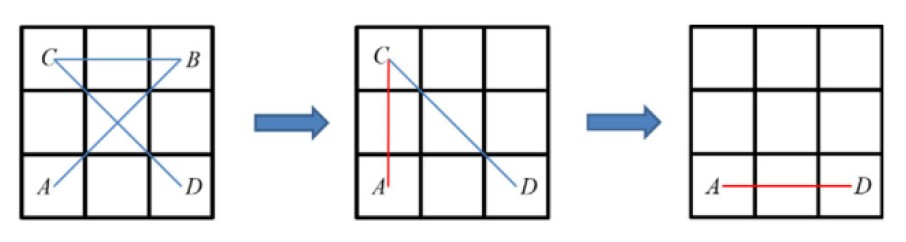
\includegraphics[scale=0.6]{cross_filter}
	\centering
	\caption{بهینه سازی  مسیر با استفاده از فیلتر \lr{P(x,y)}}
	\cite{paliwal2023survey}
	\label{crosspath:fig1}
\end{figure} 

\begin{figure}[h]
	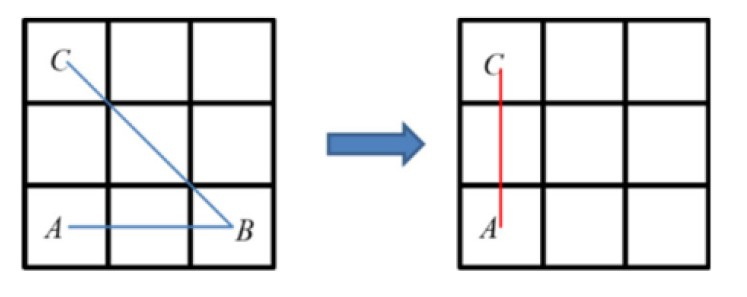
\includegraphics[scale=0.6]{sawtooth}
	\centering
	\caption{بهینه سازی  مسیر با استفاده از فیلتر \lr{W(x,y)}}
	\cite{paliwal2023survey}
	\label{sawtooth:fig2}
\end{figure}
\begin{figure}[h]
	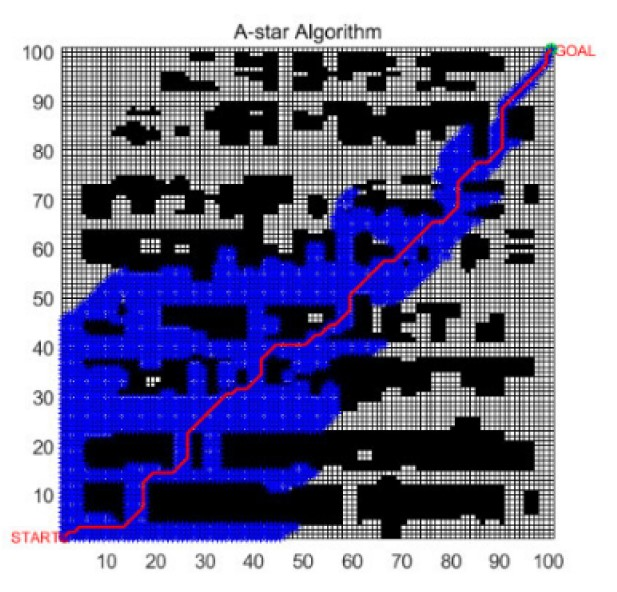
\includegraphics[scale=0.7]{a_star_vs_geo}
	\centering
	\caption{مسیر یابی توسط الگوریتم کلاسیک \lr{A*}}
	\cite{paliwal2023survey}
	\label{a_star}
	\end{figure}
	
\begin{figure}[h]
	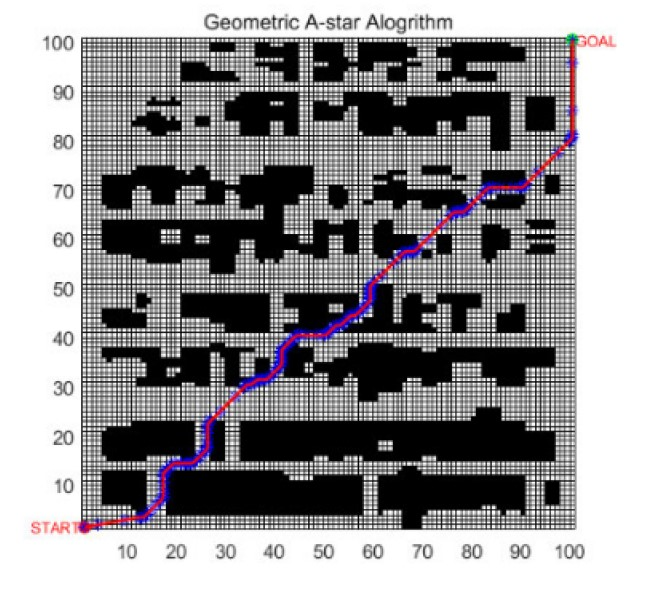
\includegraphics[scale=0.7]{geo}
	\centering
	\caption{ مسیر یابی توسط الگوریتم روش هندسی \lr{A*}}
	\cite{paliwal2023survey}
	\label{geo}
\end{figure}
\subsection{بهبودیافته}
این الگوریتم ابتدا هدف و موقعیت شروع را توسط یک خط مستقیم به هم متصل می کند. سپس فهرستی از مراکز، که نقاطی روی خط هستند که برخورد کردن به آن ها ممنوع می باشد را  ایجاد می کند. برای هر مرکز، دایره‌ای به شعاع معین \lr{r} 
در اطراف این نقاط می‌سازد، و سپس مختصات محل ها ی برخورد این دایره ها را با خط پیدا می کند به عنوان نمونه شکل 
\ref{improved}
 ر ادر نظر بگیرید . سپس با انتخاب هر یک از این جفت ها به عنوان نقطه شروع و هدف محلی، با استفاده از آستانه
  $\epsilon$
 بررسی می کند که آیا هدف محلی 
 \lr{E}
  و شروع محلی بعدی 
\lr{ I} 
 به یکدیگر نزدیک هستند یا خیر. اگر نزدیک باشند، هدف محلی فعلی به هدف محلی بعدی تغییر می کند، یعنی برنامه ریز باید مسیری را از 
 \lr{D }
 به
  \lr{K}
 ، همانطور که در شکل نشان داده شده است، برنامه ریزی کند. پس از انجام این کار، الگوریتم با استفاده از الگوریتم 
 \lr{A*}
 ، مسیرهای موضعی را در اطراف همه جفت های 
 \lr{(D,E)} 
 و 
 \lr{(D,K)}
  مسیریابی می کند.  رد نهایت مسیری حاصل می شود که بخشی از آن شامل خطی راست است که کواه ترین مسیر است و موانع با استفاده از الگوریتم
  \lr{ A*}
    دور زده می شوند .

\begin{figure}[h]
	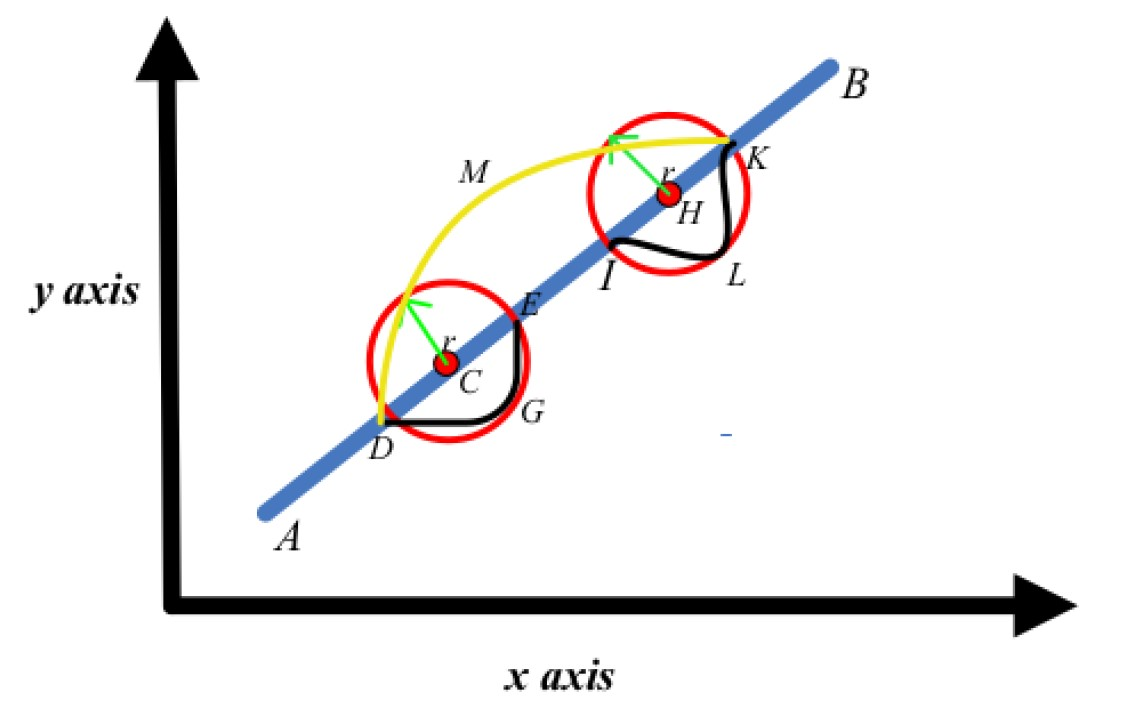
\includegraphics[scale=0.4]{improved}
	\centering
	\caption{ شیوه کار  \lr{A*}بهبود یافته}
	\cite{paliwal2023survey}
	\label{improved}
\end{figure}
\subsection{همیشه اصلاح شونده}
در  عمل ، مقدار زمان در دسترس برای محاسبه راه‌حل بدون برخورد با توجه به محیط ارائه‌شده، محدود است واین محدویت زمان بر دشواری  حل می افزاید . الگوریتم‌های \lr{Anytime} دسته‌ای از الگوریتم‌ها هستند که می‌توانند با محاسبه سریع یک راه‌حلی که لزوما بهینه نیست  شروع کنند و این جواب را به تدریج به سمت بهینگی اصلاح نمایند  الگوریتم \lr{ARA*} راه حلی برای محدودیت زمان  ارائه می دهد، بلکه بسیار کارآمد است، زیرا از تاریخچه ی جستجوی قبلی خود استفاده می کند. این موضوع  اجازه می دهد تا از محاسبه مجدد حالت های قبلی جلوگیری شود . الگوریتم از یک اکتشافی وزنی استفاده می کند، بنابراین،$ f(n) = g(n) + ε∗ h(n).$ با تنظیم 
$\epsilon=1$  
، الگوریتم کلاسیک \lr{A*} راه حل های بهینه را ارائه می دهد. برای
 $\epsilon>1$ 
، راه‌حل‌ها ممکن است بهینه نباشند . نتایج تجربی روی یک ربات نشان می دهد که رباتی که از 
\lr{4D ARA* Planner} 
استفاده می کند حدود 0.6 ثانیه طول می کشد تا به یک طرح تقریباً بهینه دست یابد. 



\subsection{پویا ساده}

الگوریتم
\lr{ D* Lite}
،مانند الگوریتم 
\lr{A* }
کلاسیک با شروع از یک گره سعی می کند تابه نقطه ی هدف برسد اما با این فرض که گراف بتواند تغییر کند . تشخیص یک مانع همان اثری را بر روی نمودار خواهد داشت که با حذف یال بین دو گره که مانع بین آنها تشخیص داده می شود، و این معادل تغییر وزن یال به ∞ است. الگوریتم
\lr{ D* Lite}
 چنین تغییرات وزنی را در نمودار محاسبه می کند و به طور مداوم مسیر خودروی خودران را دوباره برنامه ریزی می کند.
الگوریتم
\lr{D* Lite}
  دو امتیاز را برای هر گره از گراف ذر نظر می گیرد  
   \lr{G}
    و  
    \lr{RHS}
   .  که همانند 
 \lr{  A* }
   امتیاز
    \lr{G}
     هزینه رفتن از گره شروع به گره فعلی در گراف می باشد. امتیاز
    
    \lr{RHS }
    به صورت
     $RHS(n) = min(G(n′) + C(n′, n)) $
    تعریف می شود که در آن،
     \lr{n}
     گره فعلی، 
    \lr{n′} 
    گره قبلی است.  و  
   \lr{ C(n′, n)}
    هزینه جابجایی از 
    \lr{n }
    به
     \lr{n}
    . برای یافتن گره بهینه بعدی استفاده می شود. اگر گره بعدی مسدود شود،
    \lr{ C} 
    برای آن لبه روی 
    $\infty$ 
    تنظیم می شود، در نتیجه،
    \lr{ RHS}
     نیز روی 
     $\infty$
     تنظیم می شود. با استفاده از این امتیازها، الگوریتم مسیری را از هدف تا شروع برنامه‌ریزی می‌کند که در نهایت یک مسیر بهینه را برای دنبال کردن به دست می‌دهد. در صورت مواجهه با یک مانع ناشناخته قبلی، امتیاز 
     \lr{RHS }
     با هزینه های جدید اتصال برای گره های آسیب دیده، دوباره محاسبه می شود. نتایج نشان می‌دهد که
      \lr{D* Lite }
     منجر به جست و جوی راس اضافی کمتر، گسترده شدن کمتر ی می‌شود، که ثابت می‌کند که
      \lr{D* Lite}
       در واقع الگوریتم خوبی برای برنامه‌ریزی مجدد و حرکت در محیط‌های ناشناخته است.




\subsection{همیشه پویا}
محیط‌های پویا را به حساب می‌آورد، که یک مشکل عمده است که باید در برنامه‌ریزی وسایل نقلیه خودران مورد توجه قرار گیرد. از آنجایی که فرد می‌خواهد کل زمان سفر به حداقل برسد، باید برنامه‌ریز راه‌حل‌ها را با بیشترین سرعتی که می‌تواند محاسبه کند. در صورت برخورد با یک مانع جدید، زمان سفر با زمان اضافی برای محاسبه یک مسیر جدید افزایش می یابد. برای مقابله با این مشکل، الگوریتم ADA* با ترکیب ایده‌های دو الگوریتم قبلاً مورد بحث، D*lite [12] و ARA* [11] توسعه یافت. مشابه ARA*، AD* راه حل هایی با ضریب تورم کاهشی را جستجو می کند که به طور مستمر مرز زیر بهینه راه حل را بهبود می بخشد. هر تغییری که در محیط شناسایی شود (از طریق سنسور یا دوربین)، به عنوان تغییر در نموداری که مسیر در آن برنامه ریزی شده است، منعکس خواهد شد. گره‌های آسیب‌دیده در فهرست باز مانند الگوریتم D* Lite ارسال می‌شوند، با اولویت‌های آنها در میان مقدار کلید قبلی و مقدار کلید به‌روزرسانی. سپس گره های موجود در لیست پردازش می شوند تا زمانی که راه حل فعلی تضمین شود ϵ-suboptimal باشد. بنابراین ADA*، که یک الگوریتم در هر زمان است، امکان برنامه ریزی مجدد سریع راه حل ها را با محدود کردن بهینه بودن آنها فراهم می کند. شکل 13 هزینه های راه حل متحمل شده و بسط حالت انجام شده توسط A*، D* Lite و AD* را در برابر احتمال ظاهر شدن مانع نشان می دهد (این آزمایش شامل شبیه سازی یک بازوی رباتیک با 3 درجه آزادی بود که یک افکتور انتهایی را از طریق یک محیط پویا دستکاری می کرد. [13]). شکل 12 نمونه ای از یک ربات ناوبری ساده را نشان می دهد که از سلول پایین سمت راست شبکه شروع می شود و قرار است به سلول سمت چپ بالای شبکه حرکت کند. سلول های خاکستری نشان دهنده حالت های گسترش یافته توسط هر الگوریتم در موقعیت مربوطه خود هستند. ربات دو قدم به جلو حرکت می کند و شکاف دیوار بالایی را مشاهده می کند. شش الگوریتم برای برنامه ریزی مسیرهای بدون برخورد مورد استفاده قرار گرفت: A*، وزن دار A* با ε = 2.5، D* Lite، وزن دار D* Lite با 2.5 = ϵ، ARA* و AD*. جدول III نتایج را برای مثال ربات ناوبری ساده از

\section{جمع بندی}

حوزه خودروهای خودمختار پیشرفت چشمگیری داشته است، اما هنوز هم دامنه پیشرفت زیادی در آینده دارد. این مقاله در ابتدا تکنیک‌های مختلف برنامه‌ریزی حرکتی را ارائه کرد که تمرکز اصلی آن بر روی الگوریتم جستجوی \lr{A* } و تغییرات آن بود. چندین گونه از الگوریتم  \lr{A* } مورد بررسی قرار گرفت و نشان داده شد که چگونه این تغییرات به حل مسائل با الگوریتم کلاسیک \lr{ A *} کمک می کند. بسیاری از تغییرات الگوریتم  \lr{A* } را می توان در آینده با بهینه سازی الگوریتم کلاسیک یا انواع آن توسعه داد و آزمایش کرد. یکی از این تغییرات بالقوه، اصلاح تابع اکتشافی مورد استفاده در این الگوریتم‌ها است. نویسنده امیدوار است که این مقاله در ارائه یک نمای کلی از انواع مختلف الگوریتم  \lr{A* } موفق باشد، که می تواند به عنوان مرجع در حین کار بر روی انواع جدید برای ارائه عملکرد بهتر نسبت به الگوریتم های برنامه ریزی حرکتی موجود استفاده شود.





